% This file was converted to LaTeX by Writer2LaTeX ver. 1.0.2
% see http://writer2latex.sourceforge.net for more info
\documentclass[a4paper]{article}
\usepackage[utf8]{inputenc}
\usepackage[T3,T1]{fontenc}
\usepackage[english]{babel}
\usepackage[noenc]{tipa}
\usepackage{tipx}
\usepackage[geometry,weather,misc,clock]{ifsym}
\usepackage{pifont}
\usepackage{eurosym}
\usepackage{amsmath}
\usepackage{wasysym}
\usepackage{amssymb,amsfonts,textcomp}
\usepackage{color}
\usepackage{array}
\usepackage{hhline}
\usepackage{hyperref}
\hypersetup{pdftex, colorlinks=true, linkcolor=blue, citecolor=blue, filecolor=blue, urlcolor=blue, pdfsubject=, pdfkeywords=}
\usepackage[pdftex]{graphicx}
% List styles
\newcommand\liststyleLSi{%
\renewcommand\labelitemi{\ding{108}}
\renewcommand\labelitemii{o}
\renewcommand\labelitemiii{{\FilledSmallSquare}}
\renewcommand\labelitemiv{\ding{108}}
}
\newcommand\liststyleLSii{%
\renewcommand\labelitemi{\ding{108}}
\renewcommand\labelitemii{o}
\renewcommand\labelitemiii{{\FilledSmallSquare}}
\renewcommand\labelitemiv{\ding{108}}
}
% Page layout (geometry)
\setlength\voffset{-1in}
\setlength\hoffset{-1in}
\setlength\topmargin{0.9839in}
\setlength\oddsidemargin{1.1811in}
\setlength\textheight{9.7251in}
\setlength\textwidth{5.9059in}
\setlength\footskip{0.0cm}
\setlength\headheight{0cm}
\setlength\headsep{0cm}
% Footnote rule
\setlength{\skip\footins}{0.0469in}
\renewcommand\footnoterule{\vspace*{-0.0071in}\setlength\leftskip{0pt}\setlength\rightskip{0pt plus 1fil}\noindent\textcolor{black}{\rule{0.25\columnwidth}{0.0071in}}\vspace*{0.0398in}}
% Pages styles
\makeatletter
\newcommand\ps@Standard{
  \renewcommand\@oddhead{}
  \renewcommand\@evenhead{}
  \renewcommand\@oddfoot{}
  \renewcommand\@evenfoot{}
  \renewcommand\thepage{\arabic{page}}
}
\makeatother
\pagestyle{Standard}
\date{}
\begin{document}
\clearpage\setcounter{page}{1}\pagestyle{Standard}
{\centering 

\includegraphics[width=3.5693in,height=1.7807in]{Tra1n-img/Tra1n-img1.png}
\par}


\bigskip


\bigskip


\bigskip


\bigskip

{\centering\color{black}
\textbf{Tra1n}
\par}


\bigskip


\bigskip


\bigskip


\bigskip

{\raggedleft\color{black}
Antonio Carlos Falcão Petri 586692
\par}

{\raggedleft\color{black}
José Antônio dos Santos Júnior 586765
\par}

{\raggedleft\color{black}
José Vitor de Carvalho Aquino 609170
\par}

{\raggedleft\color{black}
Tiago Bonadio Badoco 586722
\par}


\bigskip


\bigskip


\bigskip


\bigskip


\bigskip


\bigskip


\bigskip


\bigskip


\bigskip


\bigskip


\bigskip


\bigskip

{\centering\color{black}
São Carlos
\par}

{\centering\color{black}
Junho/2015
\par}

{\color{black}
\textbf{Autores:}}

{\color{black}
Antonio Carlos Falcão Petri
(\href{mailto:falcaopetri@gmail.com}{falcaopetri}\href{mailto:falcaopetri@gmail.com}{@}\href{mailto:falcaopetri@gmail.com}{gmail}\href{mailto:falcaopetri@gmail.com}{.}\href{mailto:falcaopetri@gmail.com}{com})
– Implementação do Jogo}

{\color{black}
José Antônio dos Santos Júnior
(\href{mailto:jusantosjr@hotmail.com}{jusantosjr}\href{mailto:jusantosjr@hotmail.com}{@}\href{mailto:jusantosjr@hotmail.com}{hotmail}\href{mailto:jusantosjr@hotmail.com}{.}\href{mailto:jusantosjr@hotmail.com}{com})
– Desenvolvimento Gráfico}

{\color{black}
José Vitor Aquino
(\href{mailto:jvcaquino95@gmail.com}{jvcaquino}\href{mailto:jvcaquino95@gmail.com}{95@}\href{mailto:jvcaquino95@gmail.com}{gmail}\href{mailto:jvcaquino95@gmail.com}{.}\href{mailto:jvcaquino95@gmail.com}{com})
– Implementação das Estruturas de Dados}

{\color{black}
Tiago Bonadio Badoco
(\href{mailto:tiago.badoco@gmail.com}{tiago}\href{mailto:tiago.badoco@gmail.com}{.}\href{mailto:tiago.badoco@gmail.com}{badoco}\href{mailto:tiago.badoco@gmail.com}{@}\href{mailto:tiago.badoco@gmail.com}{gmail}\href{mailto:tiago.badoco@gmail.com}{.}\href{mailto:tiago.badoco@gmail.com}{com})
- \ Documentação}


\bigskip

{\color{black}
\textbf{Funcionamento do Jogo:}}

{\color{black}
No jogo, tem-se como objetivo juntar os vagões de trem à locomotiva de
acordo com a ordem determinada pela estação. Para isso, existe uma fila
de vagões onde, em ordem, tendo como primeiro elemento o vagão 1 e como
último elemento o vagão . A ordem que os vagões devem aparecer no final
(ou seja, ligados à locomotiva) é determinada de forma aleatória e
aparece na placa sobre a estação de trem.}

{\color{black}
Para montar as sequências os jogadores podem passar um trem diretamente
ou então empilhar ele na plataforma de vagões. Só é possível retirar da
plataforma de vagões o último vagão adicionado a ela. Para efetuar tais
ações temos dois semáforos e um guindaste. O semáforo da esquerda
permite os vagões irem para o centro do cenário onde podem ser levados
a plataforma por meio do guindaste ou podem passar para se acoplar à
locomotiva, isso se o semáforo da direita for acionado. Só é possível
retirar um vagão da plataforma se não houver nenhum vagão posicionado
no centro do cenário.}

{\color{black}
Nem todas as sequências propostas pela estação são factíveis. Caso o
jogador se depare com uma sequência que não pode ser efetuada ele deve
clicar no botão “Impossível montar a sequência” localizado no canto
superior direito. Caso a sequência seja factível o jogador deve acoplar
os vagões adequadamente à locomotiva. Todo esse processo deve ser feito
em 60 segundos sendo que, se o tempo estourar, é considerada uma
derrota.}

{\color{black}
Esse jogo é uma leve adaptação da situação proposta no
\href{https://www.urionlinejudge.com.br/judge/en/problems/view/1062}{Exercício}\href{https://www.urionlinejudge.com.br/judge/en/problems/view/1062}{
}\href{https://www.urionlinejudge.com.br/judge/en/problems/view/1062}{Rails}\href{https://www.urionlinejudge.com.br/judge/en/problems/view/1062}{
- 1062}, descrito no URI Online Judge. De fato, a ideia de criar o
Tra1n veio durante a tentativa de resolução de tal exercício.}


\bigskip

{\color{black}
\textbf{Controles:}}

{\color{black}
Mouse – O mouse controla todas as interações com os menus do jogo,
selecionando as opções desejadas.}

{\color{black}
Setas – Movimentam o guindaste.}

{\color{black}
“A” – Ativa o semáforo da esquerda, permitindo a ida dos vagões da fila
para a posição central do cenário.}

{\color{black}
“D” – Ativa o semáforo da direita, permitindo o acoplamento dos vagões
posicionados no centro do cenário.}

\begin{center}
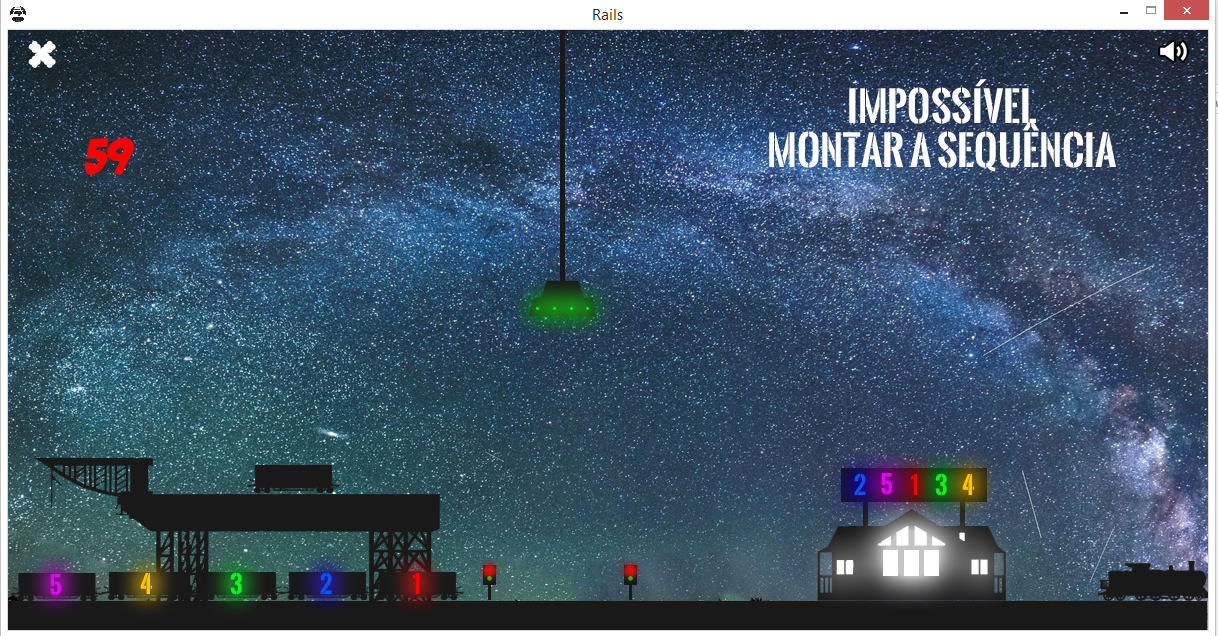
\includegraphics[width=5.2272in,height=2.7646in]{Tra1n-img/Tra1n-img2.png}
\end{center}

\bigskip


\bigskip


\bigskip

{\centering\color{black}
Imagem 1 - Tela do Jogo
\par}


\bigskip

{\color{black}
\textbf{Ferramentas:}}

\liststyleLSi
\begin{itemize}
\item {\color{black}
Codeblocks;}
\item {\color{black}
Allegro 5.0;}
\item {\color{black}
Photoshop CS5;}
\item {\color{black}
Astah Professional;}
\item {\color{black}
Fruity Loops Producer Edition 11;}
\item {\color{black}
STL, C++~Standard Template Library. }
\end{itemize}

\bigskip

{\color{black}
\textbf{TAD’s}}


\bigskip

{\color{black}
A implementação do jogo utilizada utiliza-se de 3 estruturas de dados
para organizar os principais elementos do jogo. São elas: um deque
encapsulado em uma estrutura Fila e em uma Pilha, e um Map.}

{\color{black}
É importante ressaltar que as duas estruturas implementadas utilizam o
conceito de Templates, mantendo a camada de abstração entre a estrutura
e os dados que ela armazena. Além disso, teve-se como parâmetro de
implementação as estruturas da STL, referências em C++.}


\bigskip

{\bfseries\color{black}
Deque}


\bigskip


\bigskip

{\color{black}
\ \ \textbf{D}ouble-\textbf{e}nded \textbf{que}ue ou fila duplamente
encadeada, funciona como um
\textcolor[rgb]{0.13333334,0.13333334,0.13333334}{\ container que
possui tamanho dinâmico e pode ser expandido ou contraído em ambas as
extremidades, dessa forma possuindo métodos de inserção, exclusão e
recuperação da informação em ambas as extremidades.}}


\bigskip

{\color{black}
\textbf{\textcolor[rgb]{0.13333334,0.13333334,0.13333334}{Como o Deque é
implementado?}}}


\bigskip

{\color{black}
\textcolor[rgb]{0.13333334,0.13333334,0.13333334}{O Deque é utilizado
tanto para auxiliar na construção de outras estruturas utilizadas no
jogo quanto como um tipo de Lista. Ela é implementada para inserir
elementos de forma dinâmica e duplamente encadeado. }}

{\color{black}
\textcolor[rgb]{0.13333334,0.13333334,0.13333334}{As funções de deque
utilizadas e implementadas no jogo foram: Deque(), \~{}Deque(),
pushFront(), pushBack(), popFront(), popBack(), front(), back(),
empty(), at().}}



\begin{center}
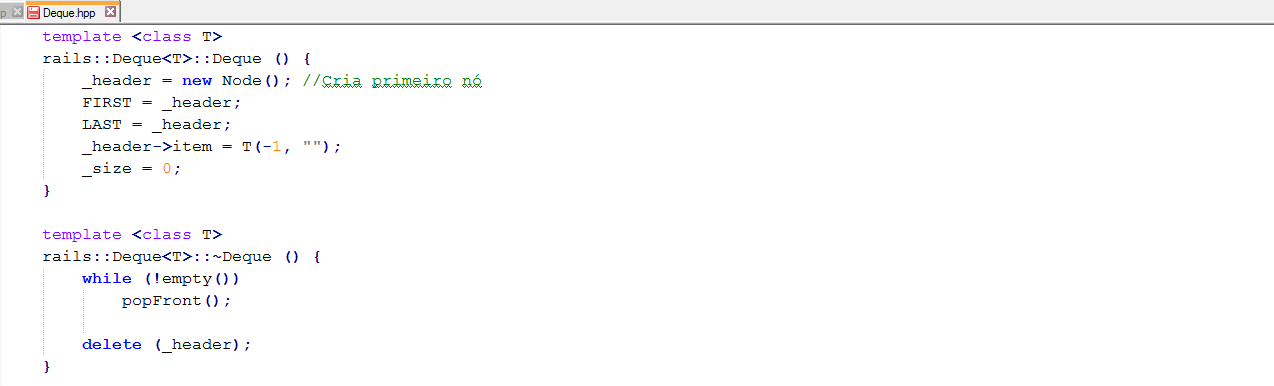
\includegraphics[width=6.2709in,height=1.9028in]{Tra1n-img/Tra1n-img3.png}
\end{center}
{\centering\color{black}
\textcolor[rgb]{0.13333334,0.13333334,0.13333334}{\ \ \ }Imagem 2 \ –
Construtor e destrutor
\par}


\bigskip

{\color{black}
\textcolor[rgb]{0.13333334,0.13333334,0.13333334}{O método construtor
cria um novo nó em Header. Como a deque está sendo inicializado, o nó a
direita(first) e o a esquerda(last) do Header será ele mesmo.
}\textcolor[rgb]{0.13333334,0.13333334,0.13333334}{\ }}

{\color{black}
\textcolor[rgb]{0.13333334,0.13333334,0.13333334}{O método destrutor,
pensando na reusabilidade e portabilidade, utiliza a função popFront()
para liberar a memória dos elementos do deque. Quando restar apenas o
nó Header, este é deletado como os outros nós.}}


\bigskip


\bigskip


\bigskip


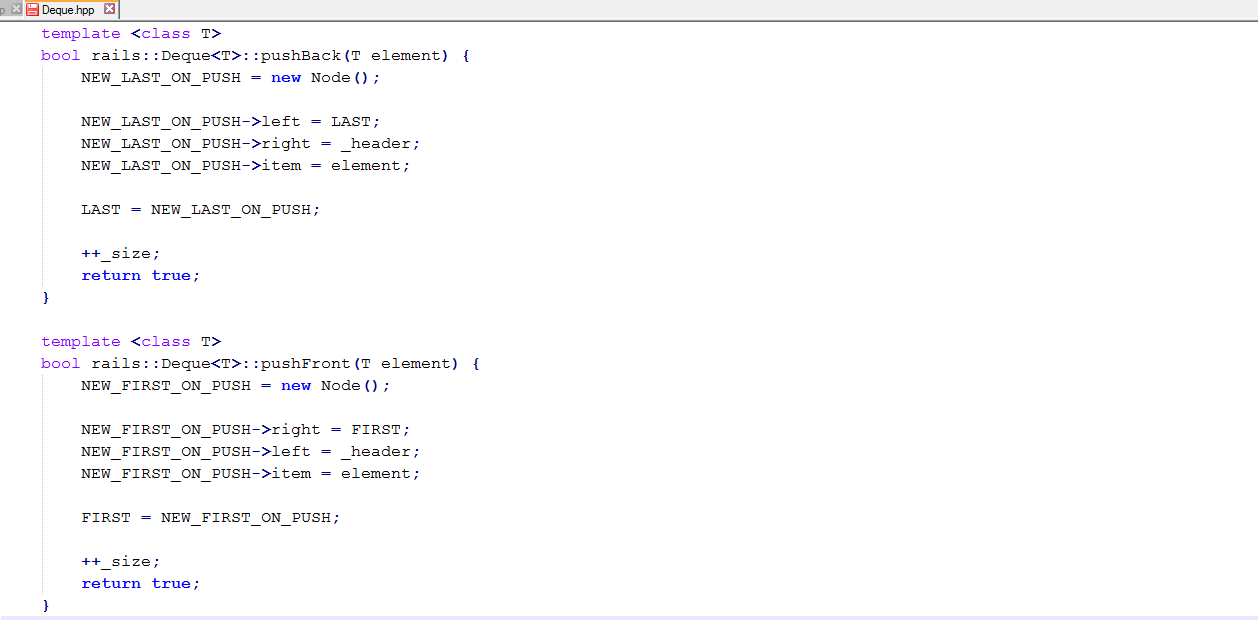
\includegraphics[width=6.2709in,height=3.0972in]{Tra1n-img/Tra1n-img4.png}


{\centering\color{black}
Imagem 3 \ – pushBack, pushFront
\par}


\bigskip

{\color{black}
\textcolor[rgb]{0.13333334,0.13333334,0.13333334}{Pensando que a
estrutura Deque é duplamente encadeada, foram criados métodos
pushBack() e pushFront(), onde podem ser utilizados para inserir
valores tanto no inicio (pushFront), quanto no final da estrutura
(pushBack).}}

{\color{black}
\textcolor[rgb]{0.13333334,0.13333334,0.13333334}{É utilizado dois
define’s para a implementação dessas funções, eles serão responsáveis
por apontar inicio e fim do deque }na inserção.}


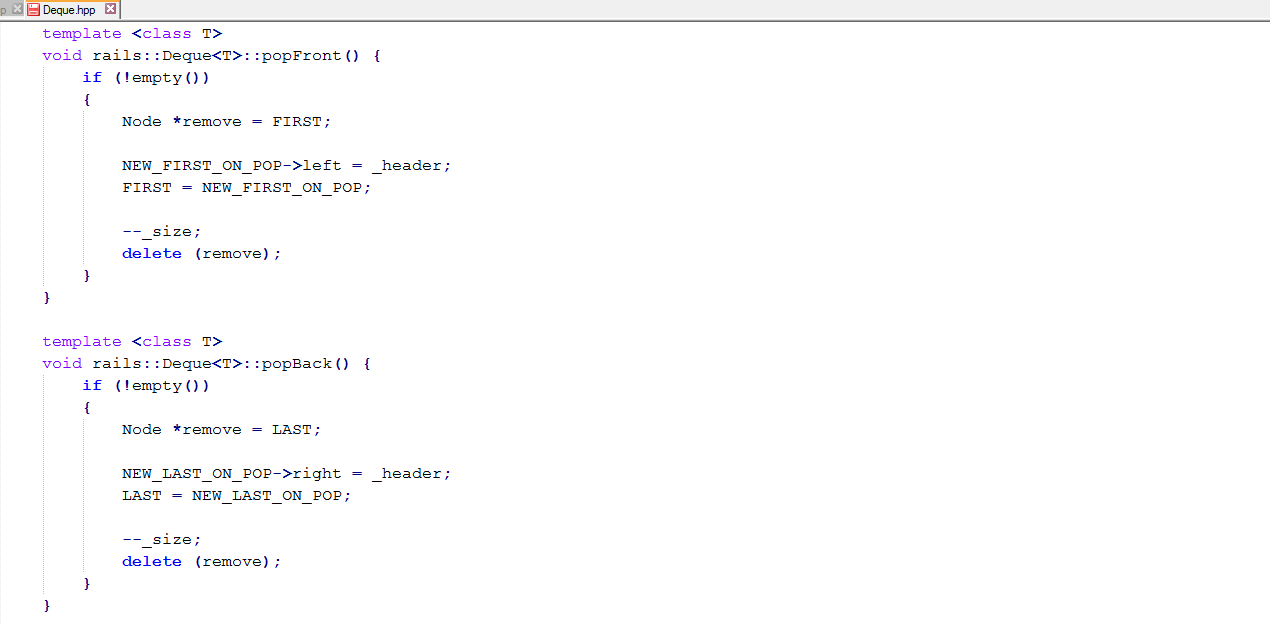
\includegraphics[width=6.2709in,height=3.0835in]{Tra1n-img/Tra1n-img5.png}


{\centering\color{black}
Imagem 4 \ – popBack, popFront
\par}


\bigskip


\bigskip

{\color{black}
\textcolor[rgb]{0.13333334,0.13333334,0.13333334}{Seguindo o conceito de
estrutura duplamente encadeada, foram criados métodos popBack() e
popFront(), onde podem ser utilizados para remover valores tanto no
inicio (popFront), quanto no final da estrutura (popBack).}}

{\color{black}
\textcolor[rgb]{0.13333334,0.13333334,0.13333334}{É utilizado dois
define’s para a implementação dessas funções, eles serão responsáveis
por apontar inicio e fim do deque }na remoção.}


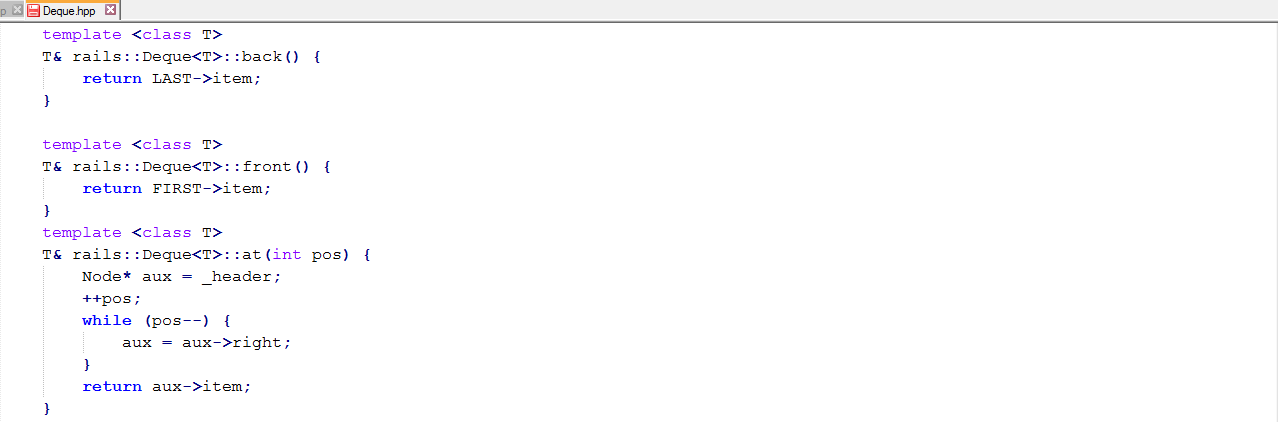
\includegraphics[width=6.2709in,height=2.0693in]{Tra1n-img/Tra1n-img6.png}


{\centering\color{black}
Imagem 5 \ – back, front, e at
\par}


\bigskip

{\color{black}
\textcolor[rgb]{0.13333334,0.13333334,0.13333334}{Back() e Front() são
implementadas utilizando os defines first e last, para setar o inicio e
o fim da estrutura, essas funções retornam o valor do primeiro elemento
(front), e último (back).}}


\bigskip

{\centering\color{black}
Imagem 6 \ – erase, size
\par}

\begin{center}
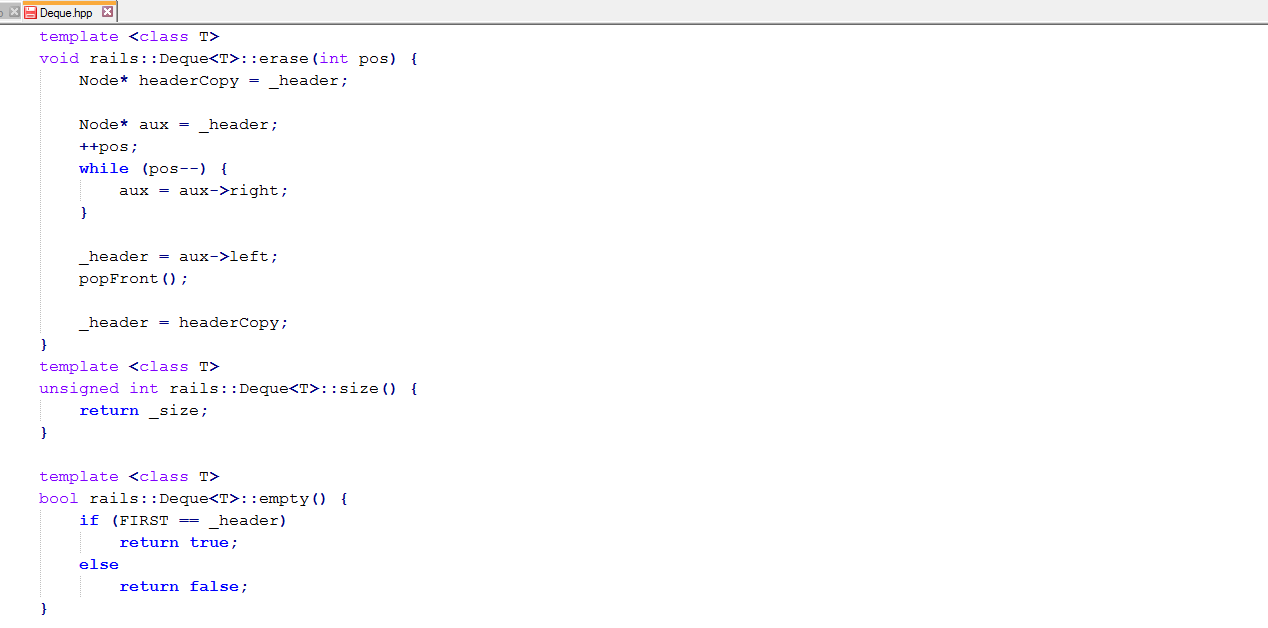
\includegraphics[width=6.2709in,height=3.111in]{Tra1n-img/Tra1n-img7.png}
\end{center}

\bigskip


\bigskip

{\color{black}
\textbf{\textcolor[rgb]{0.13333334,0.13333334,0.13333334}{Como a Fila é
implementada e utilizada?}}}


\bigskip

{\color{black}
\textcolor[rgb]{0.13333334,0.13333334,0.13333334}{A Fila é utilizada
para armazenar os vagões de 1 a 5 em ordem crescente. Ela é
implementada para inserir elementos de forma dinâmica e encadeada.
Assim, surge a utilização do Deque, onde todas as funções necessárias
para manipulação de uma fila já foram
implementadas.}\textcolor[rgb]{0.13333334,0.13333334,0.13333334}{ \ }}

{\color{black}
\textcolor[rgb]{0.13333334,0.13333334,0.13333334}{As funções de fila
utilizadas e implementadas no jogo foram: Queue(), \~{}Queue(), push(),
pop(), front(), e empty().}}


\bigskip


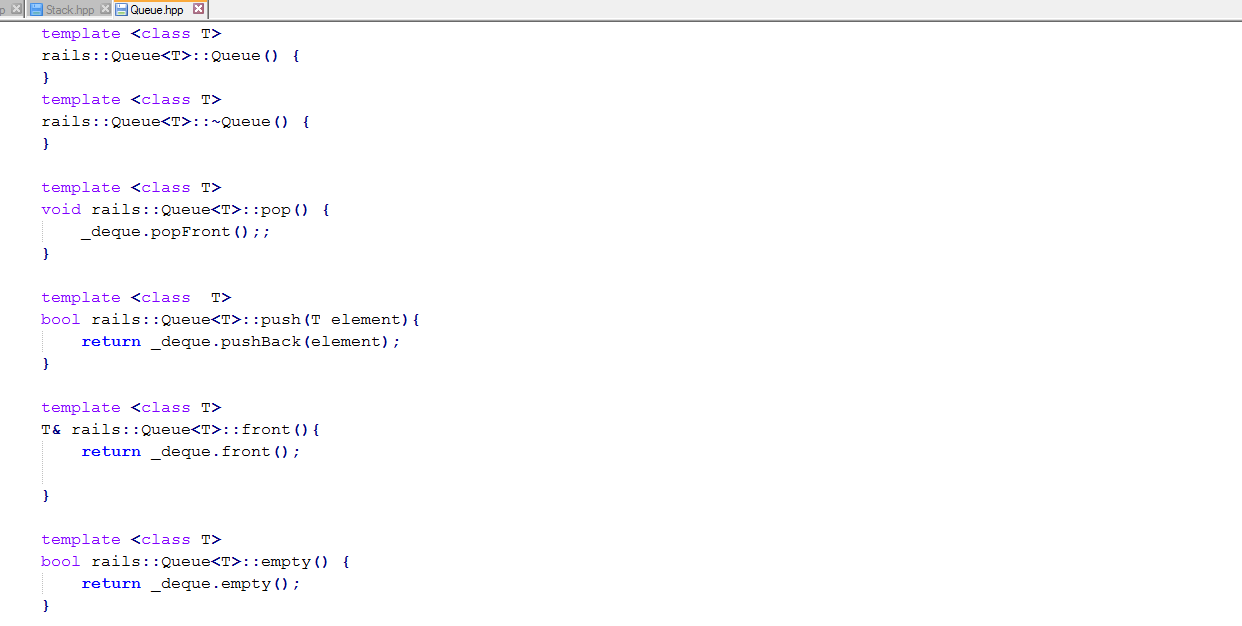
\includegraphics[width=6.2709in,height=3.1665in]{Tra1n-img/Tra1n-img8.png}


{\centering\color{black}
Imagem 7 \ – Construtor, destrutor, push, front, e empty
\par}


\bigskip


\bigskip


\bigskip

{\color{black}
\textbf{\textcolor[rgb]{0.13333334,0.13333334,0.13333334}{Como a Pilha é
implementada e utilizada?}}}


\bigskip

{\color{black}
\textcolor[rgb]{0.13333334,0.13333334,0.13333334}{A Pilha é utilizada
para armazenar os vagões que são tirados da fila inicial. Ela é
implementada para inserir elementos de forma dinâmica e encadeada.
Assim, surge a utilização do Deque, onde todas as funções necessárias
para manipulação de uma pilha já foram
implementadas.}\textcolor[rgb]{0.13333334,0.13333334,0.13333334}{ \ }}

{\color{black}
\textcolor[rgb]{0.13333334,0.13333334,0.13333334}{As funções de fila
utilizadas e implementadas no jogo foram: Stack(), \~{}Stack(), push(),
pop(), top(), e empty().}}


\bigskip

{\centering\color{black}

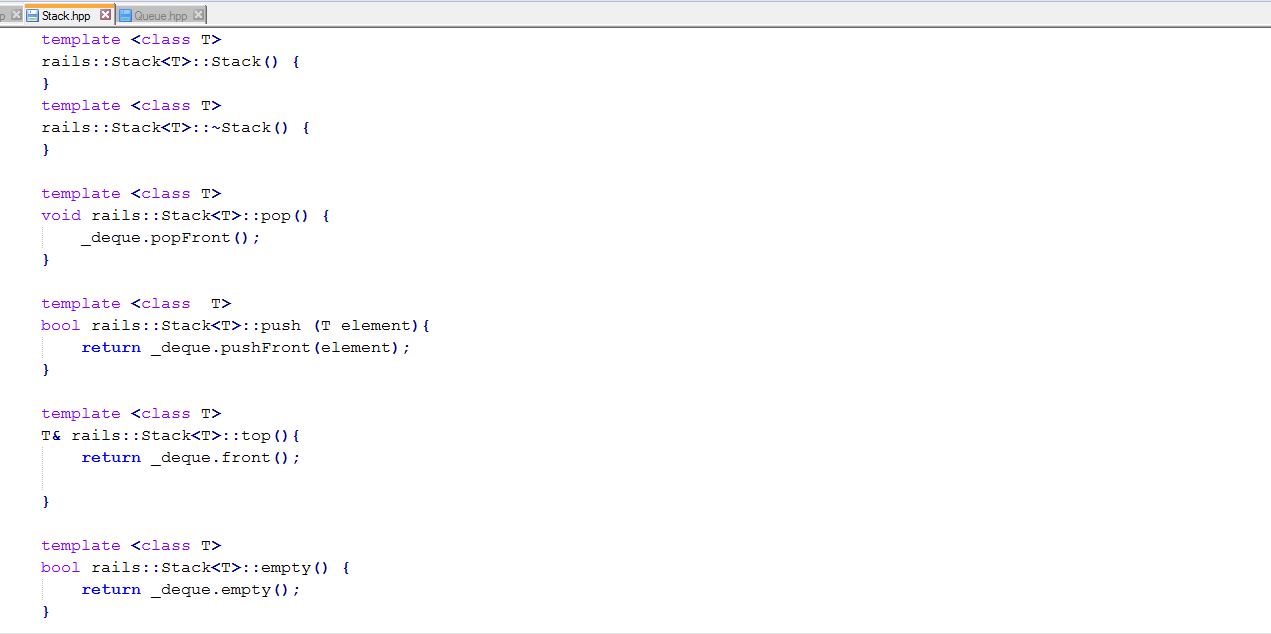
\includegraphics[width=6.2709in,height=3.1252in]{Tra1n-img/Tra1n-img9.png}
Imagem 8 \ – Construtor, destrutor, push, front, e empty
\par}


\bigskip



\begin{center}
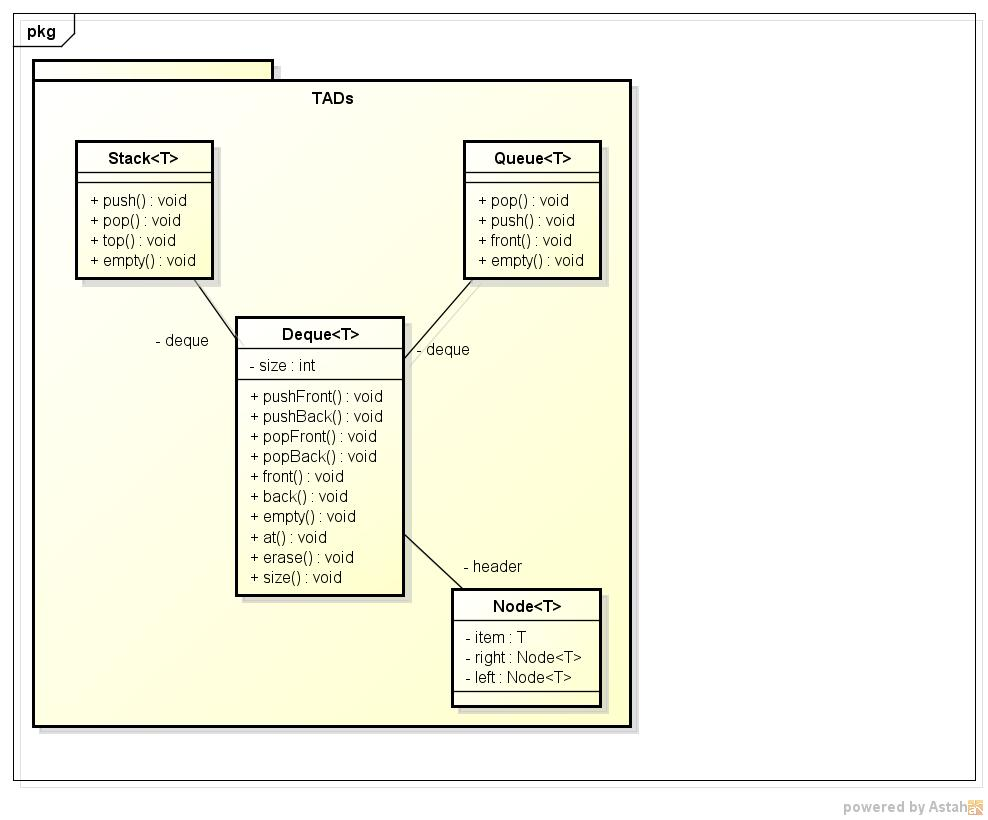
\includegraphics[width=3.7709in,height=4.1354in]{Tra1n-img/Tra1n-img10.jpg}
\end{center}

\bigskip


\bigskip


\bigskip


\bigskip


\bigskip


\bigskip


\bigskip


\bigskip


\bigskip


\bigskip


\bigskip


\bigskip


\bigskip


\bigskip


\bigskip


\bigskip


\bigskip


\bigskip


\bigskip


\bigskip

{\centering\color{black}
Imagem 9 \ – Diagrama de Classes: TADs
\par}


\bigskip

{\color{black}
\textbf{Como o Mapa é utilizado?}}

{\color{black}
Um Mapa é uma estrutura de dados que permite o armazenamento de
elementos “indexados” por uma chave, normalmente única. Externamente, e
para fins didáticos, se parece com um vetor que, ao invés de ter
índices numéricos e acessar o elemento “na posição I”, permite ter
qualquer tipo de objeto como índice e acessa o elemento “com a chave
K”.}

{\color{black}
Internamente, entretanto, os mapas possuem comportamentos diferentes.
Eles costumam ordenar seus dados em relação à chave e, para manter
eficiência nas operações de inserção, consulta e remoção, são
implementados com árvores binárias balanceadas.}

{\color{black}
Na implementação desse jogo, foi utilizado o std::map, um container da
STL. Dessa forma, pode-se definir identificadores às imagens utilizadas
e manipuladas pelo jogo. São utilizados dois maps. Um relaciona o
identificador da imagem ao endereço (relative-path) de seu arquivo no
sistema. O outro, relaciona um identificador (o mesmo, por comodidade e
coerência) à um objeto da Classe IDrawing.}

{\color{black}
Dessa forma, reúne-se todas as imagens do sistema em uma única estrutura
de dados, que assegura velocidade na manipulação desses objetos. Ex:}

{\color{black}
\textcolor[rgb]{0.8392157,0.6156863,0.52156866}{systemImages[}\textcolor[rgb]{0.3372549,0.6117647,0.8392157}{”name”}\textcolor[rgb]{0.8392157,0.6156863,0.52156866}{].}\textcolor[rgb]{0.3254902,0.5058824,0.20784314}{getBitmap}\textcolor[rgb]{0.8392157,0.6156863,0.52156866}{();}}

{\color{black}
\textbf{Arquitetura do Software: }}

{\color{black}
\ \ A disposição geral do jogo baseia-se de criação de uma RailsGUI, que
encapsula tanto as regras do jogo (Game) quanto a interpretação gráfica
dada a ele. Para tal, criou-se o conceito de Telas (Screens), que
possuem um sub-conjunto de imagens desenháveis.}

{\color{black}
\ \ Dessa forma, não é necessário identificar qual Tela atual está sendo
exibida, pois todas possuem a mesma interface (de métodos). A Tela do
Jogo (PlayScreen), por possuir uma lógica de funcionamento
diferenciada, é uma especialização de uma Screen.}

\begin{center}
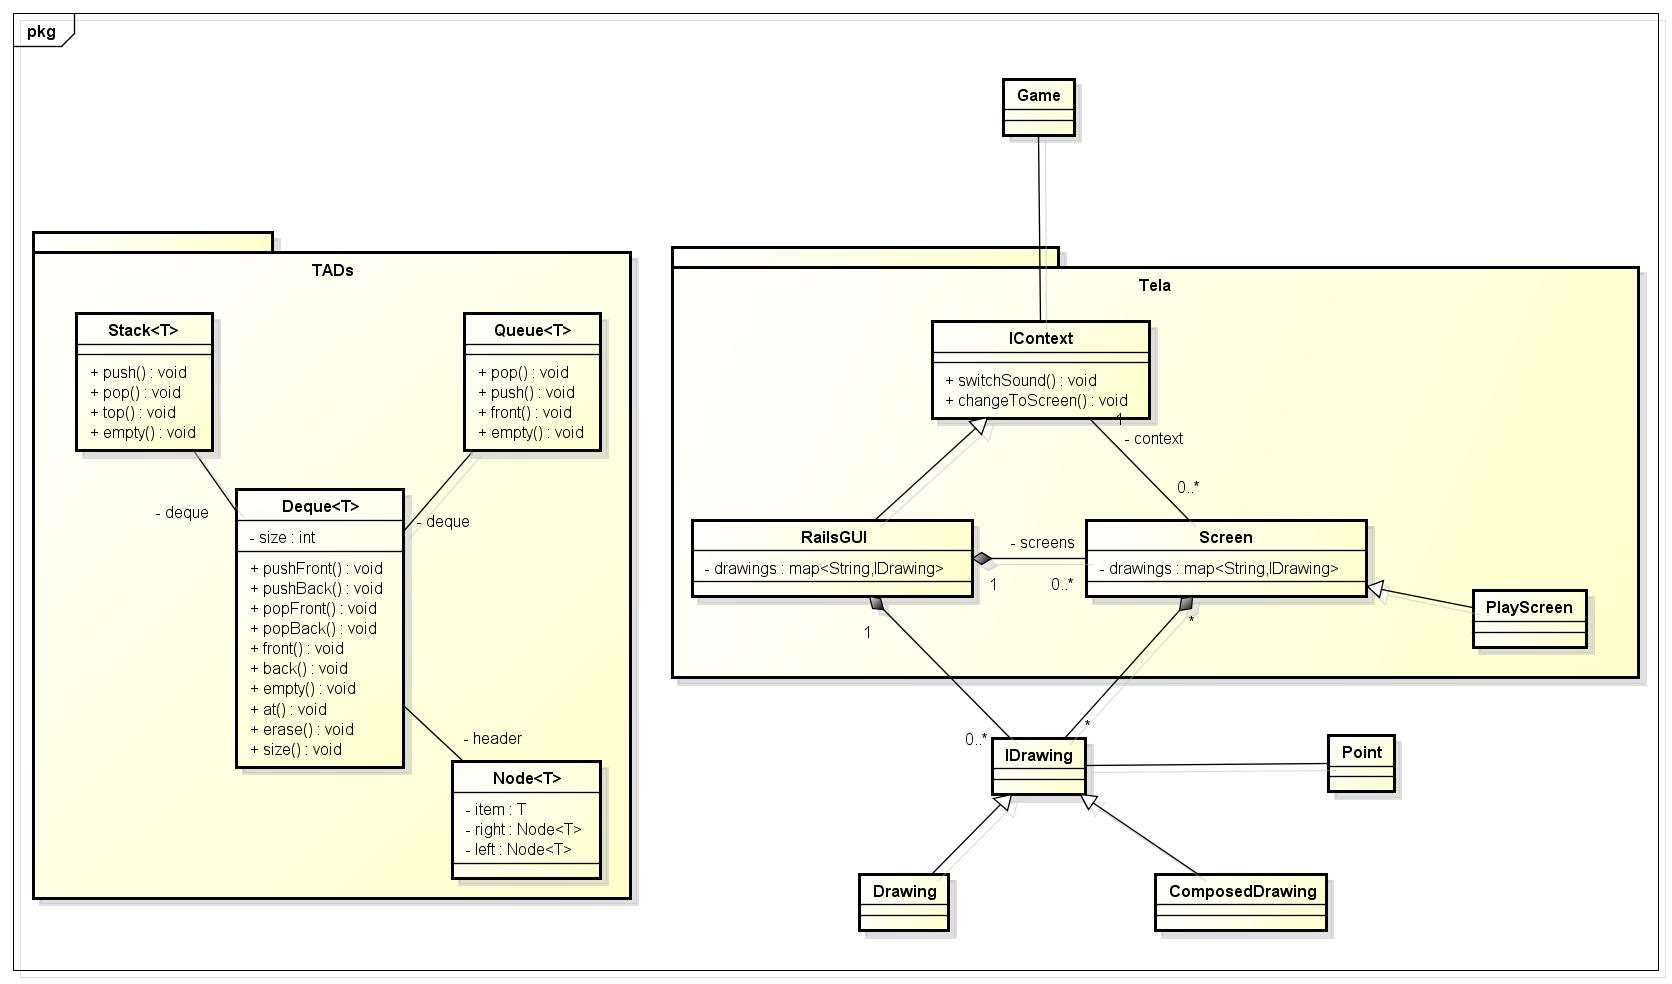
\includegraphics[width=3.5417in,height=3.1874in]{Tra1n-img/Tra1n-img11.jpg}
\end{center}

\bigskip


\bigskip


\bigskip


\bigskip


\bigskip


\bigskip


\bigskip


\bigskip


\bigskip


\bigskip


\bigskip

{\centering\color{black}
Imagem 10 \ – Diagrama de Classes: Visão simplificada do Jogo
\par}


\bigskip

{\color{black}
\textbf{Observações e Comentários:}}

{\color{black}
Essa seção reúne pequenas informações quanto ao processo de
desenvolvimento do jogo.}

\liststyleLSii
\begin{itemize}
\item {\color{black}
O Jogo em sua versão atual é dependente da dll
allegro-5.0.10-monolith-mt.dll. Vários esforços foram realizados
buscando eliminar essa necessidade. A ideia central é fazer um
static-linkage com as bilibotecas *-static-mt.dll disponibilizadas pelo
Allegro. Entretanto, não foi encontrado nenhum caso de sucesso. Outra
alternativa seria utilizar programas injetores de dlls em executáveis.
Testou-se esse procedimento com o programa PE-Inject, mas sem sucesso.
Exemplo de insucesso no static-linkage:
\href{https://www.allegro.cc/forums/thread/613981}{https}\href{https://www.allegro.cc/forums/thread/613981}{://}\href{https://www.allegro.cc/forums/thread/613981}{www}\href{https://www.allegro.cc/forums/thread/613981}{.}\href{https://www.allegro.cc/forums/thread/613981}{allegro}\href{https://www.allegro.cc/forums/thread/613981}{.}\href{https://www.allegro.cc/forums/thread/613981}{cc}\href{https://www.allegro.cc/forums/thread/613981}{/}\href{https://www.allegro.cc/forums/thread/613981}{forums}\href{https://www.allegro.cc/forums/thread/613981}{/}\href{https://www.allegro.cc/forums/thread/613981}{thread}\href{https://www.allegro.cc/forums/thread/613981}{/613981};}
\item {\color{black}
Para atribuir um ícone ao executável, seguiu-se o procedimento descrito
em
\href{https://www.allegro.cc/forums/thread/601721Monolith}{https}\href{https://www.allegro.cc/forums/thread/601721Monolith}{://}\href{https://www.allegro.cc/forums/thread/601721Monolith}{www}\href{https://www.allegro.cc/forums/thread/601721Monolith}{.}\href{https://www.allegro.cc/forums/thread/601721Monolith}{allegro}\href{https://www.allegro.cc/forums/thread/601721Monolith}{.}\href{https://www.allegro.cc/forums/thread/601721Monolith}{cc}\href{https://www.allegro.cc/forums/thread/601721Monolith}{/}\href{https://www.allegro.cc/forums/thread/601721Monolith}{forums}\href{https://www.allegro.cc/forums/thread/601721Monolith}{/}\href{https://www.allegro.cc/forums/thread/601721Monolith}{thread}\href{https://www.allegro.cc/forums/thread/601721Monolith}{/601721}\href{https://www.allegro.cc/forums/thread/601721Monolith}{Monolith};}
\item {\color{black}
Foi utilizado o addon PhysicsFS do Allegro, uma camada de abstração do
PhysicsFS, que por sua vez, permite acesso à vários tipos de arquivos.
Dessa forma, pode-se ler arquivos zipados pelos mesmos métodos de
acesso de arquivos do Allegro. Veja:
\href{https://www.allegro.cc/manual/5/physfs.html}{https}\href{https://www.allegro.cc/manual/5/physfs.html}{://}\href{https://www.allegro.cc/manual/5/physfs.html}{www}\href{https://www.allegro.cc/manual/5/physfs.html}{.}\href{https://www.allegro.cc/manual/5/physfs.html}{allegro}\href{https://www.allegro.cc/manual/5/physfs.html}{.}\href{https://www.allegro.cc/manual/5/physfs.html}{cc}\href{https://www.allegro.cc/manual/5/physfs.html}{/}\href{https://www.allegro.cc/manual/5/physfs.html}{manual}\href{https://www.allegro.cc/manual/5/physfs.html}{/5/}\href{https://www.allegro.cc/manual/5/physfs.html}{physfs}\href{https://www.allegro.cc/manual/5/physfs.html}{.}\href{https://www.allegro.cc/manual/5/physfs.html}{html};}
\item {\color{black}
Utilizou-se a função setResourceArchive() no arquivo TheLastTooFast.cpp.
Tal função está descrita em
\href{https://www.allegro.cc/forums/thread/614268}{https}\href{https://www.allegro.cc/forums/thread/614268}{://}\href{https://www.allegro.cc/forums/thread/614268}{www}\href{https://www.allegro.cc/forums/thread/614268}{.}\href{https://www.allegro.cc/forums/thread/614268}{allegro}\href{https://www.allegro.cc/forums/thread/614268}{.}\href{https://www.allegro.cc/forums/thread/614268}{cc}\href{https://www.allegro.cc/forums/thread/614268}{/}\href{https://www.allegro.cc/forums/thread/614268}{forums}\href{https://www.allegro.cc/forums/thread/614268}{/}\href{https://www.allegro.cc/forums/thread/614268}{thread}\href{https://www.allegro.cc/forums/thread/614268}{/614268},
e faz com que o working-directory da aplicação seja mudado para a pasta
em que se encontra o executável. Assim, pode-se utilizar relative-paths
para referenciar os arquivos usados pelo jogo;}
\item {\color{black}
A Arquitetura de Screens proposta não foi suficiente para a
representação abstrata de uma Tela, tendo-se que criar artifícios
internos para a correta manipulação dos elementos. De toda forma, ela
pode ser revista e refinada, possivelmente, enquadrando-a em um Design
Pattern.}
\end{itemize}

\bigskip
\end{document}
